\documentclass[12pt, twoside]{article}
\input{../preamble}
\usepackage{float}

\title{Physics}
\author{Chris Huson}
\date{April 2026}

\fancyhead[LE]{\thepage}
\fancyhead[RO]{\thepage \\ First \& last name: \hspace{2.25cm} \,\\  \,}
\fancyhead[LO]{La Scuola d'Italia / Huson / Physics \\* 13 April 2026}

\begin{document}

\subsubsection*{3.1 Classwork: Vector Addition}

\begin{enumerate}[itemsep=0.3cm]

\item Two vectors $\vec{A}$ and $\vec{B}$ are drawn from the origin. Using the \textbf{head-to-tail method}, find the resultant $\vec{R} = \vec{A} + \vec{B}$. Show your construction and draw the resultant on the grid.

\begin{center}
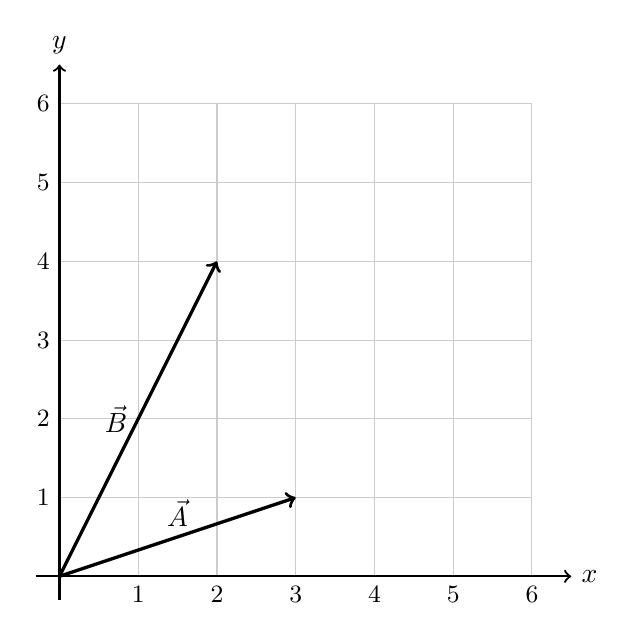
\begin{tikzpicture}[scale=1]
  \draw[gray!40, thin, step=1] (0,0) grid (6,6);
  \draw[->, thick] (-0.3,0) -- (6.5,0) node[right]{$x$};
  \draw[->, thick] (0,-0.3) -- (0,6.5) node[above]{$y$};
  \foreach \x in {1,...,6} \node[below] at (\x,0) {\small \x};
  \foreach \y in {1,...,6} \node[left] at (0,\y) {\small \y};
  % Vector A = (3,1)
  \draw[->, very thick] (0,0) -- (3,1) node[midway, above]{$\vec{A}$};
  % Vector B = (2,4)
  \draw[->, very thick] (0,0) -- (2,4) node[midway, left]{$\vec{B}$};
  % Solution — uncomment to see the answer
  %\draw[->, thick, dashed] (3,1) -- (5,5) node[midway, right]{\small $\vec{B}$};
  %\draw[->, very thick] (0,0) -- (5,5) node[near end, above left]{$\vec{R}$};
\end{tikzpicture}
\end{center}

$\vec{R} = (\hspace{1.5cm},\hspace{1.5cm})$

\item The same two vectors are drawn below. Using the \textbf{parallelogram method}, find the resultant $\vec{R} = \vec{A} + \vec{B}$. Complete the parallelogram and draw the resultant as the diagonal from the origin.

\begin{center}
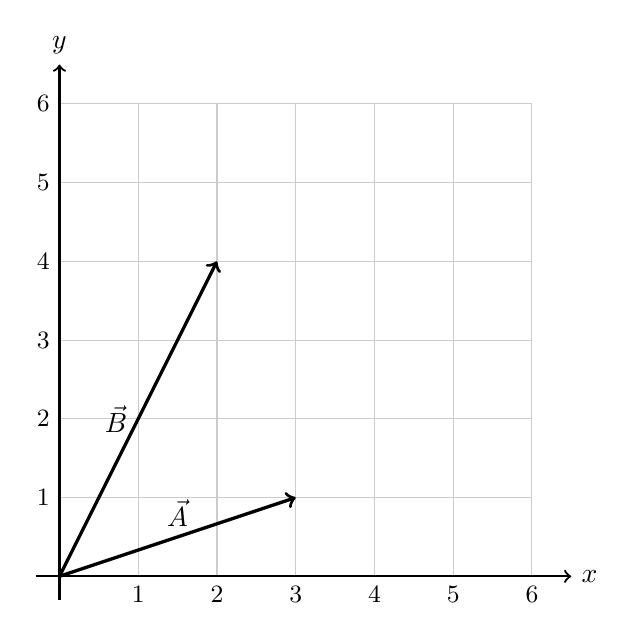
\begin{tikzpicture}[scale=1]
  \draw[gray!40, thin, step=1] (0,0) grid (6,6);
  \draw[->, thick] (-0.3,0) -- (6.5,0) node[right]{$x$};
  \draw[->, thick] (0,-0.3) -- (0,6.5) node[above]{$y$};
  \foreach \x in {1,...,6} \node[below] at (\x,0) {\small \x};
  \foreach \y in {1,...,6} \node[left] at (0,\y) {\small \y};
  % Vector A = (3,1)
  \draw[->, very thick] (0,0) -- (3,1) node[midway, above]{$\vec{A}$};
  % Vector B = (2,4)
  \draw[->, very thick] (0,0) -- (2,4) node[midway, left]{$\vec{B}$};
  % Solution — uncomment to see the answer
  %\draw[thick, dashed] (3,1) -- (5,5);
  %\draw[thick, dashed] (2,4) -- (5,5);
  %\draw[->, very thick] (0,0) -- (5,5) node[near end, above left]{$\vec{R}$};
\end{tikzpicture}
\end{center}

$\vec{R} = (\hspace{1.5cm},\hspace{1.5cm})$

\newpage

\item Draw vectors $\vec{C} = (4,\, 2)$ and $\vec{D} = (1,\, 3)$ from the origin on the grid below. Find $\vec{R} = \vec{C} + \vec{D}$ using either the head-to-tail or parallelogram method. Show your construction and draw the resultant.

\begin{center}
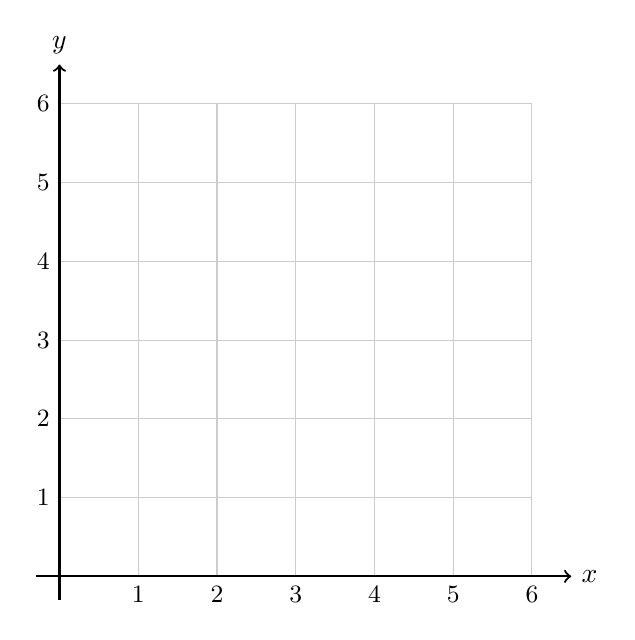
\begin{tikzpicture}[scale=1]
  \draw[gray!40, thin, step=1] (0,0) grid (6,6);
  \draw[->, thick] (-0.3,0) -- (6.5,0) node[right]{$x$};
  \draw[->, thick] (0,-0.3) -- (0,6.5) node[above]{$y$};
  \foreach \x in {1,...,6} \node[below] at (\x,0) {\small \x};
  \foreach \y in {1,...,6} \node[left] at (0,\y) {\small \y};
  % Solution — uncomment to see the answer
  %\draw[->, very thick] (0,0) -- (4,2) node[midway, below right]{$\vec{C}$};
  %\draw[->, very thick] (0,0) -- (1,3) node[midway, above left]{$\vec{D}$};
  %\draw[->, thick, dashed] (4,2) -- (5,5) node[midway, right]{\small $\vec{D}$};
  %\draw[->, very thick] (0,0) -- (5,5) node[near end, above left]{$\vec{R}$};
\end{tikzpicture}
\end{center}

$\vec{R} = (\hspace{1.5cm},\hspace{1.5cm})$

%\vspace{1cm}

\item Two vectors $\vec{P}$ and $\vec{Q}$ are drawn on the grid below. Find $\vec{P} - \vec{Q}$ geometrically: draw the opposite of $\vec{Q}$ (that is, $-\vec{Q}$), then add it to $\vec{P}$ using the head-to-tail method. Draw the resultant.

\begin{center}
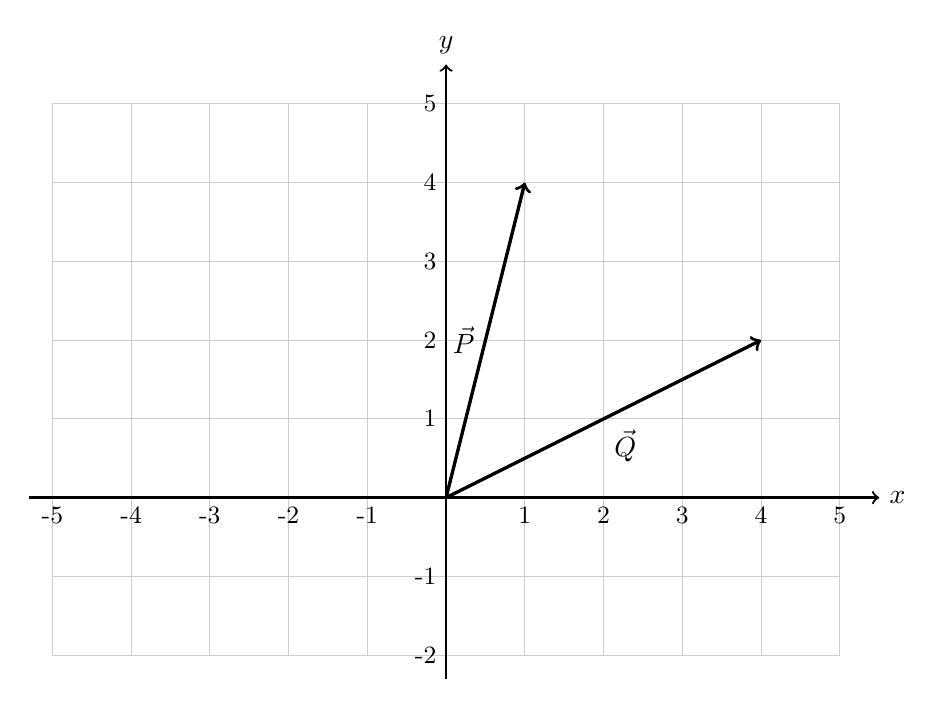
\begin{tikzpicture}[scale=1]
  \draw[gray!40, thin, step=1] (-5,-2) grid (5,5);
  \draw[->, thick] (-5.3,0) -- (5.5,0) node[right]{$x$};
  \draw[->, thick] (0,-2.3) -- (0,5.5) node[above]{$y$};
  \foreach \x in {-5,-4,...,-1,1,2,...,5} \node[below] at (\x,0) {\small \x};
  \foreach \y in {-2,-1,1,2,3,4,5} \node[left] at (0,\y) {\small \y};
  % Vector P = (1,4)
  \draw[->, very thick] (0,0) -- (1,4) node[midway, left]{$\vec{P}$};
  % Vector Q = (4,2)
  \draw[->, very thick] (0,0) -- (4,2) node[midway, below right]{$\vec{Q}$};
  % Solution — uncomment to see the answer
  % -Q = (-4, -2); place at tip of P for head-to-tail
  %\draw[->, thick, dashed] (1,4) -- (-3,2) node[midway, above]{\small $-\vec{Q}$};
  %\draw[->, very thick] (0,0) -- (-3,2) node[near end, above left]{$\vec{R}$};
\end{tikzpicture}
\end{center}

$\vec{P} - \vec{Q} = (\hspace{1.5cm},\hspace{1.5cm})$

\end{enumerate}
\end{document}
